\subsection{Prototype}

\subsubsection{Objetivo}

Especificar tipos de objetos usando uma instância prototípica a partir da qual serão criadas cópias da mesma.

\subsubsection{Motivação}

Considere-se uma framework para criação de editores gráficos de partituras:

\centerline{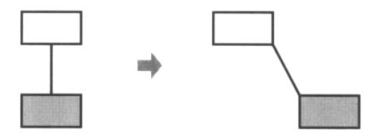
\includegraphics[scale=.7]{img/prototype/motivation.png}}

A classe GraphicTool necessita de componentes gráficos, como por exemplo notas musicais. Estas têm diversas variantes pelo que criar uma subclasse para cada uma pode ser impraticável. Nestes caso, uma alternativa mais adequada será obter novas instâncias da mesma classe a partir de um método Clone() e inicializá-las com diferentes \textit{bitmaps} e durações.

\subsubsection{Aplicação}

Usar quando:
\begin{itemize}
\item as classes a instanciar são especificadas em tempo de execução;
\item se pretende evitar ter uma hierarquia de classes \textit{factory} extensa;
\item instâncias de uma classe apenas podem ter algumas combinações de estado e, por isso, é mais conveniente clonar um protótipo e alterar parte do seu estado do que criar uma nova instância e inicializar todo o seu estado.
\end{itemize}

\subsubsection{Estrutura}

\centerline{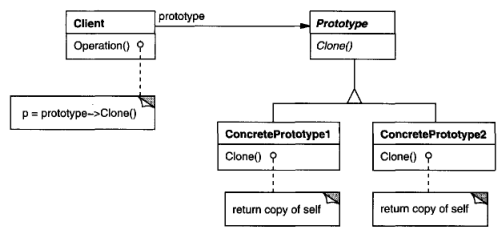
\includegraphics[scale=.7]{img/prototype/structure.png}}

\subsubsection{Participantes}
\begin{itemize}
\item Prototype (Graphic), declara uma interface para criar clones
\item ConcretePrototype (Staff, WholeNote, HalfNote), implementa o método de clonagem
\item Client (GraphicTool), cria novos objetos a partir do protótipo
\end{itemize}

\subsubsection{Colaborações}

Um cliente solicita a um protótipo cópias do mesmo.

\subsubsection{Consequências}
\begin{itemize}
\item Permite incorporar facilmente novas classes concretas de um produto num sistema de uma forma mais flexível relativamente aos restantes padrões de criação porque o cliente pode adicionar e remover protótipos em tempo de execução.
\item Permite reduzir significativamente o número de classes que um sistema necessita.
\end{itemize}

\subsubsection{Implementação}
\begin{itemize}
\item Quando o número de protótipos é dinâmico devemos considerar a utilização de um gestor de protótipos a partir do qual o cliente possa obter e guardar os protótipos.
\item Ao implementar a operação Clone devemos ter em atenção as referências a outros objetos.
\item Se o objeto a clonar não disponibilizar métodos para alterar o seu estado, pode ser necessário adicionar um método Initialize que aceite os parâmetros a inicializar como argumentos.
\end{itemize}